\documentclass[12pt]{standalone}
\usepackage{tikz}
\usetikzlibrary{positioning}
\begin{document}
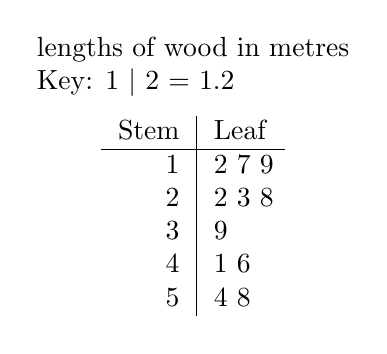
\begin{tikzpicture}
\node[align=left] (top_node) at (0,0){lengths of wood in metres \\ Key: 1 $\vert$ 2 = 1.2};
\node[below=of top_node,yshift=10mm] {
\begin{tabular}{r|l@{\hspace{4 pt}}}
Stem & Leaf\\
\hline
1 & 2 7 9 \\2 & 2 3 8 \\3 & 9 \\4 & 1 6 \\5 & 4 8 \\
\end{tabular}};
\end{tikzpicture}
\end{document}